\documentclass{article}

\usepackage[utf8]{inputenc}
\usepackage[ngerman]{babel}
\usepackage{amssymb}
\usepackage{amsmath}
\usepackage{graphics}
% Pseudocode
\usepackage{algorithm}
\usepackage[noend]{algpseudocode}
\usepackage{graphicx}

\setlength{\parindent}{0in}

\newcommand{\zettelNummer}{7}
\newcommand{\studierenderEins}{Eli Kogan-Wang (7251030)}
\newcommand{\studierenderZwei}{David Noah Stamm (7249709)}
\newcommand{\studierenderDrei}{Daniel Heins (7213874)}
\newcommand{\studierenderVier}{Tim Wolf (7269381)}

\newcounter{AufgabenCounter}
\setcounter{AufgabenCounter}{1}
\newcounter{TeilaufgabenCounter}
\newenvironment{aufgabe}{\section*{Aufgabe \theAufgabenCounter}\setcounter{TeilaufgabenCounter}{1}}{\stepcounter{AufgabenCounter}}
\newenvironment{teilaufgabe}{\paragraph*{\alph{TeilaufgabenCounter})}}{\stepcounter{TeilaufgabenCounter}}

\renewcommand{\to}{\textnormal{ to }}
\newcommand{\bigO}{\mathcal{O}}

\newcommand{\qed}{\hfill$\square$}

\begin{document}

\title{Datenstrukturen und Algorithmen \\ Heimübung \zettelNummer{}}
\author{\studierenderEins{} \\
  \studierenderZwei{} \\
  \studierenderDrei{} \\
  \studierenderVier{}}

\maketitle

% Aufgabe 1
\begin{aufgabe}
  \begin{teilaufgabe}
    Es gibt 2 Möglichkeiten dies zu implementieren:\\
    Möglichkeit 1:\\
    Push = Enqueue.
    $O(1)$\\

    Pop:
    Enqueue(Q,Dequeue(Q)) $n-1$-Mal, dann return Dequeue(Q).
    $O(n)$\\

    Möglichkeit 2:\\
    Pop = Dequeue.
    $O(1)$\\

    Push:
    Enqueue(Q,x), dann Enqueue(Dequeue(Q),x) $n-1$-Mal.
    $O(n)$\\

    Ähnlich wie bei c).

  \end{teilaufgabe}
  \begin{teilaufgabe}
    $n$ ist die Anzahl der Speicherplätze im Array.

    $a$ ist die Anzahl der Elemente im Stack $A$.
    $b$ ist die Anzahl der Elemente im Stack $B$.\\
    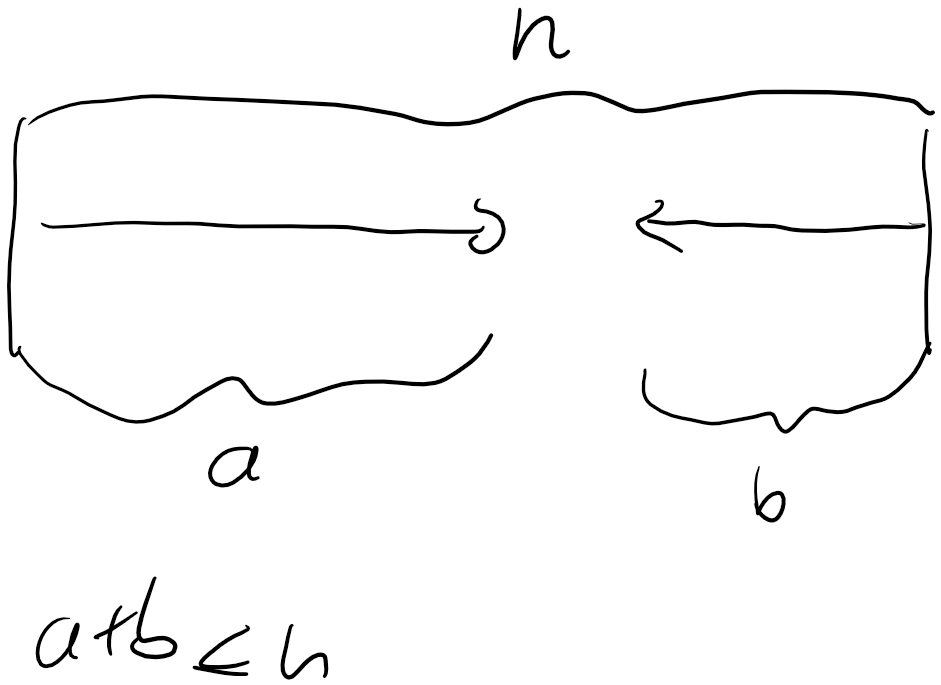
\includegraphics[width=\textwidth]{2022-05-28-Blatt-8-1-b.png}\\

    $A$ wächst nach rechts, $B$ wächst nach links.\\
  \end{teilaufgabe}
  \begin{teilaufgabe}
    Im allgemeinen ist es Möglich alle Objekte einer Qeue in einem der Stacks zu speichern.
    Der zweite Stack wird hierbei nur jeweils benötigt, um eine der Beiden Queue operationen Dequeue oder Enqueue zu realiesieren. \\
    Folglich gibt es zwei Möglichkeiten dies beiden zu implementieren: \\
    Sei $S_1$ der Stack in dem die Elemente der Queue gespeichert sind. \\
    Möglichkeit 1:
    Dequeue ist in diesem Fall identisch zu Pop und hat somit eine Laufzeit von $\mathcal{O}(1)$ \\
    Für Enqueue muss der ganze Stack mit Pop und Push Operationen in den zweiten Stack übertragen werden.
    Hierbei wird die Reihenfolge der Elemente invertiert. Nun wird das neue Objekt mit einer Push Operation hinzugefügt.
    Dannach werden wieder alle Objekte in Stack 1 übertragen und die Operation ist beendet. \\
    Da jede Push und Pop operation eine Laufzeit von $\mathcal{O}(1)$ hat liegt Enqueue in $\mathcal{O}(n)$ \\
    Möglichkeit 2:
    Enqueue ist in diesem Fall identisch zu Push und hat somit eine Laufzeit von $\mathcal{O}(1)$ \\
    Für Dequeue muss der ganze Stack mit Pop und Push Operationen in den zweiten Stack übertragen werden.
    Hierbei wird die Reihenfolge der Elemente invertiert. Nun wird das neue Objekt mit einer Pop-Operation hinzugefügt.
    Dannach werden wieder alle Objekte in Stack 1 übertragen und die Operation ist beendet. \\
    Da jede Push und Pop operation eine Laufzeit von $\mathcal{O}(1)$ hat liegt Dequeue in $\mathcal{O}(n)$ \\
  \end{teilaufgabe}
\end{aufgabe}

% Aufgabe 2
\begin{aufgabe}
  \begin{teilaufgabe}
    Die Logik beim Vorgehen bei einer Rechtsrotation ist identisch. \\
    \begin{algorithm}[H]
      \caption{Linksrotation (T,x)}
      \begin{algorithmic}[1]
        \State y $\gets$ rc[x]
        \State rc[x] $\gets$ lc[x]
        \State
        \If{lc[y] $\neq$ nil}
        \State p[y] $\gets$ p[x]
        \EndIf
        \If{$p[x] = nil$}
        \State root[T] $\gets$ y
        \ElsIf {x = lc[p[x]]}
        \State lc[p[x]] $\gets$ y
        \Else
        \State rc[p[x]] $\gets$  y
        \EndIf
        \State lc[y] $\gets$  x
        \State rc[x] $\gets$  y
        \State h[x] $\gets$ 1 + max\{h[lc[x]],h[rc[x]]\}
        \State h[y] $\gets$ 1 + max\{h[lc[y]],h[rc[y]]\}
        \State size[x] $\gets$ 1 + size[lc[x]] + size[rc[x]]
        \State size[y] $\gets$ 1 + size[lc[y]] + size[rc[y]]
      \end{algorithmic}
    \end{algorithm}
    Wobei size[nil] = 0.
    \begin{algorithm}
      \caption{SizeOf(T,x)}
      \begin{algorithmic}[1]
        \State \textbf{Return} size[x]
      \end{algorithmic}
    \end{algorithm}
  \end{teilaufgabe}
  \begin{teilaufgabe}
    Der Algortihmus wird mit der Wurzel des Baumes aufgerufen. \\
    \begin{algorithm}[H]
      \caption{k-median(T,x,k)}
      \begin{algorithmic}[1]
        \If{$SizeOf(rc[x]) - SizeOf(x) = k \lor lc[x] = rc[x]=Nil $}
        \State return x
        \EndIf
        \If{$SizeOf(lc[x]) > k-1$ }
        \State return k-median$(T,rc[x],SizeOf(x)-(SizeOf(rc[x]+1))$
        \Else
        \State return k-median$(T,lc[x],k)$
        \EndIf
      \end{algorithmic}
    \end{algorithm}
    Budget Laufzeitanalyse: \\
    Der Algorithmus ist rekursiv und ruft sich selber wieder über das linke oder rechte Kind des aktuellen Elements. Da dem Algorithmus zu Beginn die Wurzel vom Baum übergeben wird,kommt es im worst case zu h Rekursions aufrufen(,wobei h die höhe des Baumes ist) und die Laufzeit pro Aufruf ist kostant.
    Folglich hat der Algorithmus eine Laufzeit von $\mathcal{O}(h))$. Da der Betrachtete Baum ein AVL-Baum ist, ist nach Satz 12.2 gilt h = $\Theta(log(n))$. Also hat der Algorithmus eine Laufzeit von $\mathcal{O}(log(n))$
  \end{teilaufgabe}

\end{aufgabe}

% Aufgabe 3
\begin{aufgabe}
  Jeder Knoten im Baum hat eine zusätzliche Variable size, wie in 2 \\
  Auch ist jeder Knoten annotiert mit $min$ und $max$, welche das Minimum und das Maximums des Teilbaums des Knoten enthält.\\
  Erstaufruf mit $x=root[T]$\\
  \begin{algorithm}[H]
    \caption{Schnittmengensuche(T,x,a,b)}
    \begin{algorithmic}[1]
      \If {a > b}
      \State \textbf{Return} 0 $\label{terminate:a>b}$
      \EndIf
      \If {x = nil}
      \State \textbf{Return} 0 \label{terminate:x=nil}
      \EndIf
      \If {key[x] < a}
      \State \textbf{Return} Schnittmengensuche$(T,rc[x],a,b)$ \label{recurse:key[x]<a}
      \ElsIf {key[x] > b}
      \State \textbf{Return} Schnittmengensuche$(T,lc[x],a,b)$ \label{recurse:key[x]>b}
      \Else
      \State $min \gets MinimumSuche(x)$
      \State $max \gets MaximumSuche(x)$
      \If {$key[min] \leq a \land b \leq key[max]$}
      \State \textbf{Return} $size[x]$ \label{terminate:key}
      \Else
      \State $result \gets 1$ \label{result}
      \State $result \gets result$ + Schnittmengensuche$(T,lc[x],a,b)$
      \State $result \gets result$ + Schnittmengensuche$(T,rc[x],a,b)$
      \State \textbf{Return} $result$
      \EndIf
      \EndIf
    \end{algorithmic}
  \end{algorithm}

  Die Idee ist, dass wir die Schnittmengensuche mithilfe der Annotierten Variablen $size, min, max$ frühstmöglich beenden können.
  Und damit nur den Baum so tief ablaufen, bis das Ergebnis Klar ist.\\

  Unsere Laufzeit ist durch Teilbäume begrenzt, dessen Eltern-Knoten nicht im Intervall liegen.

  Da der AVL Baum balanciert und ein Binärer Suchbaum ist, befinden sich diese Teilbäume maximal auf der Höhe $\leq \log(n)$.\\
  Damit rekursieren wir uns maximal $\log(n)$ mal.\\
  Mit einer Addition von Laufzeit $O(1)$ pro Ebene ist die Laufzeit $\mathcal{O}(log(n))$.\\


  Der Algorithmus ist korrekt, da er ab Zeile $\ref{result}$ die Anzahl der Schnittmengen klassisch Berechnet, mit einer regulären Termination
  in Zeile $\ref{terminate:a>b}$ und in Zeile $\ref{terminate:x=nil}$.
  Die Rekursion in Zeile $\ref{recurse:key[x]<a}$ und in Zeile $\ref{recurse:key[x]>b}$ ist korrekt, da die Schnittmengen nur in den Teilbäumen liegen
  die links oder rechts sind.
  Die Termination mit Size in Zeile $\ref{terminate:key}$ ist korrekt, da die der gesamt Teilbaum im gesuchten Intervall liegt.
\end{aufgabe}
\end{document}
